\section{测地曲率和测地线}

通常我们把欧式平面看作是二维平直空间 (Gauss 曲率为零),而把给定第一基本形式的抽象曲面称为二维弯曲空间. 本章的目标就是研究二维弯曲空间中的几何学.

\subsection{Motivation}

对于正则参数曲面 $S$ 满足方程 $\boldsymbol{r}=\boldsymbol{r}(u^{1},u^{2})$. $C$ 是曲面 $S$ 上的一条曲线,它的方程是 $u^{\alpha}=u^{\alpha}(s),\alpha=1,2$,其中 $s$ 是曲线 $C$ 的弧长参数. 那么 $C$ 的参数方程为
\[
\boldsymbol{r}=\boldsymbol{r}(s)=\boldsymbol{r}(u^{1}(s),u^{2}(s))
\]
我们的目的是沿着曲线 $C$ 建立一个新的正交标架场 $\{ \boldsymbol{r};\boldsymbol{e}_{1},\boldsymbol{e}_{2},\boldsymbol{e}_{3} \}$,兼顾 $C$ 和 $S$ ,定义如下
\[
\boldsymbol{e}_{1}=\boldsymbol{\alpha}(s)\qquad \boldsymbol{e}_{3}=\boldsymbol{n}(s)\qquad \boldsymbol{e}_{2}=\boldsymbol{e}_{3}\times \boldsymbol{e}_{1}=\boldsymbol{n}(s)\times\boldsymbol{\alpha}(s)
\]
直观上,$\boldsymbol{e}_{2}$ 是将曲线 $C$ 的切向量 $\boldsymbol{e}_{1}=\boldsymbol{\alpha}$ 绕着 $S$ 的单位法向量 $\boldsymbol{n}$ 正向旋转 $90\degree$ 得到的. 改标架场沿着曲线 $C$ 的运动公式为
\[
\begin{cases}  
\begin{aligned}
\frac{\mathrm{d} \boldsymbol{r}(s)}{\mathrm{d} s} & = &  \boldsymbol{e}_1 , & \\
\frac{\mathrm{d} \boldsymbol{e}_1}{\mathrm{~d} s} & = & \kappa_g \boldsymbol{e}_2 & +\kappa_n \boldsymbol{e}_3, \\
\frac{\mathrm{~d} \boldsymbol{e}_2}{\mathrm{~d} s} & =-\kappa_g \boldsymbol{e}_1  &  & +\tau_g \boldsymbol{e}_3, \\
\frac{\mathrm{~d} \boldsymbol{e}_3}{\mathrm{~d} s} & =-\kappa_n \boldsymbol{e}_1 & -\tau_g \boldsymbol{e}_2, & 
\end{aligned}
\end{cases}
\]
其中 $\kappa_n e_3$ 是曲线 $C$ 的曲率向量在曲面 $S$ 的法向量上的正交投影,故 $\kappa_n$ 恰好是曲面 $S$ 上的曲线 $C$ 的\textbf{法曲率};$\kappa_g e_2$ 是曲线 $C$ 的曲率向量在曲面 $S$ 的切平面上的正交投影。这里的 $\kappa_g$ 的计算公式是
\[
\begin{aligned}
\kappa_g & =\frac{\mathrm{d}^2 \boldsymbol{r}(s)}{\mathrm{d} s^2} \cdot \boldsymbol{e}_2=\boldsymbol{r}^{\prime \prime}(s) \cdot\left(\boldsymbol{n}(s) \times \boldsymbol{r}^{\prime}(s)\right) \\
& =\left(\boldsymbol{n}(s), \boldsymbol{r}^{\prime}(s), \boldsymbol{r}^{\prime \prime}(s)\right),
\end{aligned}
\]
把最后的式子展开得到
\[
\kappa_g=\sqrt{g_{11} g_{22}-\left(g_{12}\right)^2}\begin{vmatrix}
\frac{\mathrm{d} u^1}{\mathrm{~d} s} & \frac{\mathrm{~d}^2 u^1}{\mathrm{~d} s^2}+\Gamma_{\alpha \beta}^1 \frac{\mathrm{~d} u^\alpha}{\mathrm{d} s} \frac{\mathrm{~d} u^\beta}{\mathrm{d} s} \\
\frac{\mathrm{~d} u^2}{\mathrm{~d} s} & \frac{\mathrm{~d}^2 u^2}{\mathrm{~d} s^2}+\Gamma_{\alpha \beta}^2 \frac{\mathrm{~d} u^\alpha}{\mathrm{d} s} \frac{\mathrm{~d} u^\beta}{\mathrm{d} s}
\end{vmatrix} .
\]
曲线 $C$ 作为曲面 $S$ 内的曲线的\textbf{测地曲率} $\kappa_g$ 和它作为空间曲线的曲率 $\kappa$ 的关系式是
\[
\kappa_g=\kappa \cos \tilde{\varphi}, \quad \kappa^2=\kappa_g^2+\kappa_n^2
\]
这里 $\tilde{\varphi}$ 是曲线 $C$ 的次法向量和曲面 $S$ 的单位法向量之间的夹角.

沿曲线 $C$ 的上述正交标架场的运动公式中的 $\tau_g$ 不是属于曲面的内蕴几何学的量,它的计算公式是
\[
\tau_g=\frac{1}{\sqrt{g_{11} g_{22}-\left(g_{12}\right)^2}}\begin{vmatrix}
\left(\frac{\mathrm{d} u^2}{\mathrm{~d} s}\right)^2 & -\frac{\mathrm{d} u^1}{\mathrm{~d} s} \frac{\mathrm{~d} u^2}{\mathrm{~d} s} & \left(\frac{\mathrm{~d} u^1}{\mathrm{~d} s}\right)^2 \\
g_{11} & g_{12} & g_{22} \\
b_{11} & b_{12} & b_{22}
\end{vmatrix}
\]
称为曲线的\textbf{测地挠率}. 实际上,测地挠率 $\tau_{g}$ 和法曲率 $\kappa _n$ 的性质相同,都是曲面 $S$ 在任意一点的切方向的函数,与曲线 $C$ 本身的弯曲性无关.

\subsection{测地线}

\begin{definition}[测地线]
在曲面 $S$ 上\underline{测地曲率恒等于零}的曲线称为曲面 $S$ 上的测地线. 曲面 $S$ 上的测地线是属于曲面 $S$ 的内蕴几何学的概念.
\end{definition}
因为平面曲线的测地曲率就是它的相对曲率,因此平面上的测地线就是该平面上的直线.由此可见,曲面上的测地线的概念是平面上的直线概念的推广.

\subsubsection{运动学的观点}

曲面 $S$ 上的测地线 $C$ 作为 $S$ 的外围空间 $E^3$ 中的曲线的特征是:或者曲线 $C$ 本身是直线,或者它的主法向量处处是曲面 $S$ 的法向量.从运动学观点来看,测地线 $C$ 的特征是:如果在曲面 $S$ 上运动的质点 $p$ 只受到将它约束在曲面 $S$ 上的力的作用(即作用力的方向垂直于曲面 $S$ ),则点 $p$ 的轨迹 $C$ 是曲面 $S$ 上的测地线.

\subsubsection{最短弧长}

曲面 $S$ 上的测地线 $C$ 所满足的内在特征是:对于它在曲面 $S$ 内的任意一个有固定端点的变分 $C_t(-\varepsilon<t<\varepsilon)$ 而言,$C\left(=C_0\right)$ 的弧长是变分曲线 $C_t$ 的弧长的临界值.

\subsection{曲面分类}

\begin{figure}[H]
\centering
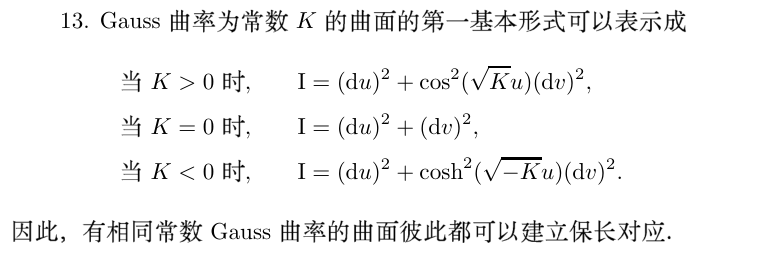
\includegraphics[width=\textwidth]{测地曲率和测地线(计算版本)-2025040401.png}
% \caption{}
\label{}
\end{figure}

\subsection{Gauss-Bonnet 公式\&定理}

\begin{figure}[H]
\centering
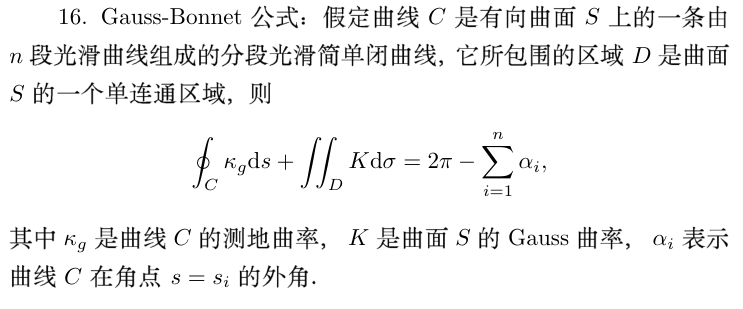
\includegraphics[width=\textwidth]{1-测地曲率和测地线(计算版本)-2025040401.png}
% \caption{}
\label{}
\end{figure}
\begin{figure}[H]
\centering
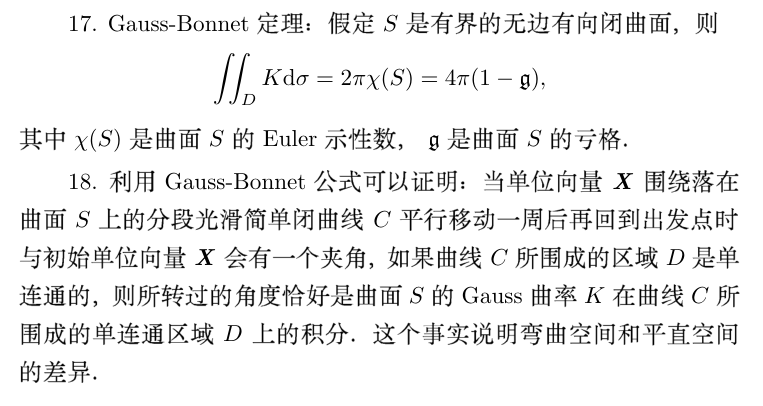
\includegraphics[width=\textwidth]{2-测地曲率和测地线(计算版本)-2025040401.png}
% \caption{}
\label{}
\end{figure}
